\documentclass[12pt,a4paper]{article}

% =============================================================================
% PACKAGES & CONFIGURATION
% =============================================================================
\usepackage[utf8]{inputenc}       % Input encoding
\usepackage[T1]{fontenc}          % Font encoding
\usepackage{lmodern}              % High-quality font
\usepackage[margin=25mm]{geometry} % Margins
\usepackage{graphicx}             % Including diagrams (BPMN, charts)
\usepackage{amsmath,amssymb,amsfonts} % Math environments
\usepackage{booktabs}             % Academic-grade tables
\usepackage{tabularx}             % Flexible tables
\usepackage{caption}              % Caption customizations
\usepackage{hyperref}             % Clicking navigation links
\usepackage{listings}             % Source code formatting
\usepackage{xcolor}               % Coloring code blocks
\usepackage{svg}
\usepackage{placeins}

% Define custom colors for Python syntax
\definecolor{codegreen}{rgb}{0.11, 0.64, 0.22}
\definecolor{codegray}{rgb}{0.47, 0.47, 0.47}
\definecolor{codepurple}{rgb}{0.58, 0, 0.82}
\definecolor{backcolor}{rgb}{0.96, 0.96, 0.96}
\definecolor{codeblue}{rgb}{0.13, 0.29, 0.53}

% Define the Python style
\lstdefinestyle{pythonstyle}{
	backgroundcolor=\color{backcolor},   
	commentstyle=\color{codegreen}\itshape,
	keywordstyle=\color{codeblue}\bfseries,
	numberstyle=\tiny\color{codegray},
	stringstyle=\color{codepurple},
	basicstyle=\ttfamily\small,
	breakatwhitespace=false,         
	breaklines=true,                 
	captionpos=b,                    
	keepspaces=true,                 
	numbers=left,                    
	numbersep=5pt,                  
	showspaces=false,                
	showstringspaces=false,
	showtabs=false,                  
	tabsize=4,
	language=Python,
	frame=single, % Adds a frame around the code
	rulecolor=\color{codegray!30}
}

% Set the default style
\lstset{style=pythonstyle}

\hypersetup{
	colorlinks=true,
	linkcolor=blue,
	urlcolor=cyan,
	pdftitle={Queue Model Implementation Report}
}

% =============================================================================
% DOCUMENT DETAILS
% =============================================================================
\begin{document}
	
	% --- Custom Title Block ---
	\begin{center}
		{\Large \textbf{Queue Model Implementation}}	 \\[0.1cm]
		{\large \textbf{Practical Session Report}} \\[0.2cm]
		{\normalsize Universitat Politécinca de Catalunya - FIB} \\[0.6cm]
		
		\begin{minipage}{0.45\textwidth}
			\flushleft \small
			\textbf{Prepared by:} \\
			Joel González Jiménez \\
		\end{minipage}
		\hfill
		\begin{minipage}{0.45\textwidth}
			\flushright \small
			\textbf{Date:} June 18, 2026 \\
			\textbf{Course:} SMDE
		\end{minipage}
		\rule{\textwidth}{0.4pt}
	\end{center}
	
	\vspace{0.3cm}
	
	% =============================================================================
	% 1. EXECUTIVE SUMMARY
	% =============================================================================
	\section{Executive Summary}
	\label{sec:summary}
	% Provide a brief and concise description of what is going to be analyzed, the problem, and the solution proposed.
	As blockchain networks experience exponential growth in transaction volumes, efficiency and processing speed have become critical challenges for network viability. This report analyzes the performance bottlenecks within the complete block lifecycle, from the initial mining phase to final verification, using an event-driven task-scheduling simulation engine. Utilizing a fractional factorial Design of Experiments (DoE), we systematically evaluate key operational factors to identify the optimal parameter configuration that maximizes block validation throughput.
	
	% =============================================================================
	% 2. SYSTEM DESCRIPTION & INTRODUCTION
	% =============================================================================
	\section{System Description and Introduction}
	\label{sec:system_description}
	% Only contains the description of the system to be modeled (not the problem, not data).
	
	The system is a simplification of a blockchain network, instead of transactions we consider that blocks arrive to the network, the nodes mine the blocks, then they broadcast the block mined to peers, finally the block is validated and consolidated in the chain.\\
	
	\noindent The simulated system contains three queues sequentially connected $(Queue1 \to Queue2 \to Queue3)$ each one with an associated task with predefined service time (10, 6, 7) respectively, the amount of servers in each queue are (c, 1, 1) being 'c' a parameter affected by a factor.
	
	\subsubsection*{BPMN Mapping}
	
	\begin{itemize}
		\item \textbf{Entry Events:} Represent the arrival of pre-compiled blocks containing transaction batches. The inter-arrival times are modeled using an exponential distribution ($M$).
		\item \textbf{Lanes:} Each lane maps directly an isolated queue within the system.
		\item \textbf{Service Tasks:} The pipeline comprises three distinct execution tasks. For architectural simplicity, the service times for all tasks follow continuous uniform distributions ($U$), with each task maintaining its own dedicated waiting queue:
		\begin{enumerate}
			\item \textbf{Task 1 --- Mining (M/U/c):} block mining and preparation.
			\item \textbf{Task 2 --- Broadcasting (U/U/1):} Network propagation of the mined block to peer nodes.
			\item \textbf{Task 3 --- Validation (U/U/1):} Cryptographic verification of the block and chain consolidation.
		\end{enumerate}
		\item \textbf{Routing Dynamics:} To facilitate the validation, the structure is configured as a sequential, multi-stage queueing network. 
	\end{itemize}
	
	\subsubsection*{Simulation Focus}
	
	The primary simulation focus centers on evaluating the system throughput, defined as the rate of validated blocks successfully appended to the blockchain upon completing the three-stage processing pipeline.
	
	% =============================================================================
	% 3. PROBLEM DESCRIPTION
	% =============================================================================
	\section{Problem Description}
	\label{sec:problem_description}
	% Describe the problem you want to solve using simulation. Clear and concise.
	
	\subsubsection*{Factors in the system}
	The simulated system is affected by four quantitative factors, table \ref{tab:factors} shows which aspects of the simulation are affected by each factor of the simulation model. 
	
%	\begin{itemize}
%		\item \textbf{Block Difficulty.} Determines the difficulty of all the blocks to be mined during the simulation.
%		\item \textbf{Peers.} Amount of servers for the mining task.
%		\item \textbf{Block Data.} Indicates the amount of data that contains each block and has to be validated.
%		\item \textbf{Block Interarrival Rate.} The interarrival rate of blocks in the system.
%	\end{itemize}
	
	\begin{table}[htbp]
		\centering
		\begin{tabular}{llll}
			\toprule
			\textbf{Name} & \textbf{Affected Element/s} & \textbf{Affected Parameter/s} & \textbf{Equation/s}\\
			\midrule
			Block Difficulty & Task1 & service time & (\ref{eq:service time task1})\\
			Peers & Task1 \& Task2 & servers \& service time &  (\ref{eq:servers task1}) \& (\ref{eq:service time task2})\\
			Block Data & Task3 & service time & (\ref{eq:service time task3})\\
			Block Interarrival Rate & Entry Events & arrival rate & (\ref{eq:arrival rate}) \\
			\bottomrule
		\end{tabular}
		\caption{Factors impact in the system.}
		\label{tab:factors}
	\end{table}
	
	The equations of the impact of factors to model parameters are the following:
	
	\begin{equation}
		\text{Task1 service time} = \text{service time} * (\text{Block Difficulty} / 10)
		\label{eq:service time task1}
	\end{equation}
	
	\begin{equation}
		\text{Task1 servers} = \text{servers} * \text{Peers}
		\label{eq:servers task1}
	\end{equation}
	
	\begin{equation}
		\text{Task2 service time} = \text{service time} * (\text{Peers} / 10)
		\label{eq:service time task2}
	\end{equation}
	
	\begin{equation}
		\text{Task3 service time} = \text{service time} * (\text{Block Data} / 20)
		\label{eq:service time task3}
	\end{equation}
	
	\begin{equation}
		\text{arrival rate}(\lambda) = \frac{1}{\text{Block Interarrival Rate}}
		\label{eq:arrival rate}
	\end{equation}\\
	
	\subsubsection*{Problem thought before simulation}
	\noindent The objective in this simulation is to maximize the throughput of blocks validation, but in this configuration the mining process could be a huge bottleneck if both factors 'Peers' and 'Block Difficulty' are unfavorable. While a higher value of 'Peers' is better for lowering the number of elements in Queue1, it is worse for Queue2, so a problem will be finding a good balance.
	
	\subsubsection*{Problem found after simulation}
	After the execution we found that 'Peers' factor had a significant impact on the block validation throughput, but the positive effect on Queue1 congestion was much important than the negative one to Queue2, so the optimum value of 'Peers' would be higher than the middle one. Also we found that factor 'Block Difficulty' and 'Block Interarrival Rate' had big impact and they are a problem if their value is high, the lower the better.
	
	\subsection{Hypotheses Framework}
	To complete the system bounds, the structural behavior, parameters, and limitations are framed under the explicit identifiers listed below:
	
	\begin{description}
		\item[\textbf{SH\_01 (Simplifying Hypothesis):}] Deviation of service times are always a 10\% of the service time
		\item[\textbf{SH\_02 (Simplifying Hypothesis):}] Transactions don't enter in a queue if the server is free.
		\item[\textbf{SH\_03 (Simplifying Hypothesis):}] There are not delays in the system.
		\item[\textbf{SH\_04 (Simplifying Hypothesis):}] All blocks have the same difficulty defined by the 'Block Difficulty' factor.
		\item[\textbf{SS\_01 (Systemic Structural):}] The queue order is First-In-First-Out ($FIFO$).
		\item[\textbf{SS\_02 (Systemic Structural):}] The capacity of the system and queues are infinite.
		\item[\textbf{SD\_01 (Systemic Data):}] Job arrival distributions ($A$) are assumed to follow a exponential distribution.
		\item[\textbf{SD\_02 (Systemic Data):}] Tasks service times follow a Uniform distribution.
		\item[\textbf{SD\_03 (Systemic Data):}] All servers associated with a Queue have a determined base service time which would be altered by factors.
		\item[\textbf{SD\_04 (Systemic Data):}] To calculate the average wait time in a queue we take into account the transactions that didn't enter the queue with zero wait time.
	\end{description}
	
	% =============================================================================
	% 4. MODEL SPECIFICATION
	% =============================================================================
	
	\section{Model Specification}
	\label{sec:model_specification}
	
	\begin{figure}[htbp]
		\centering
		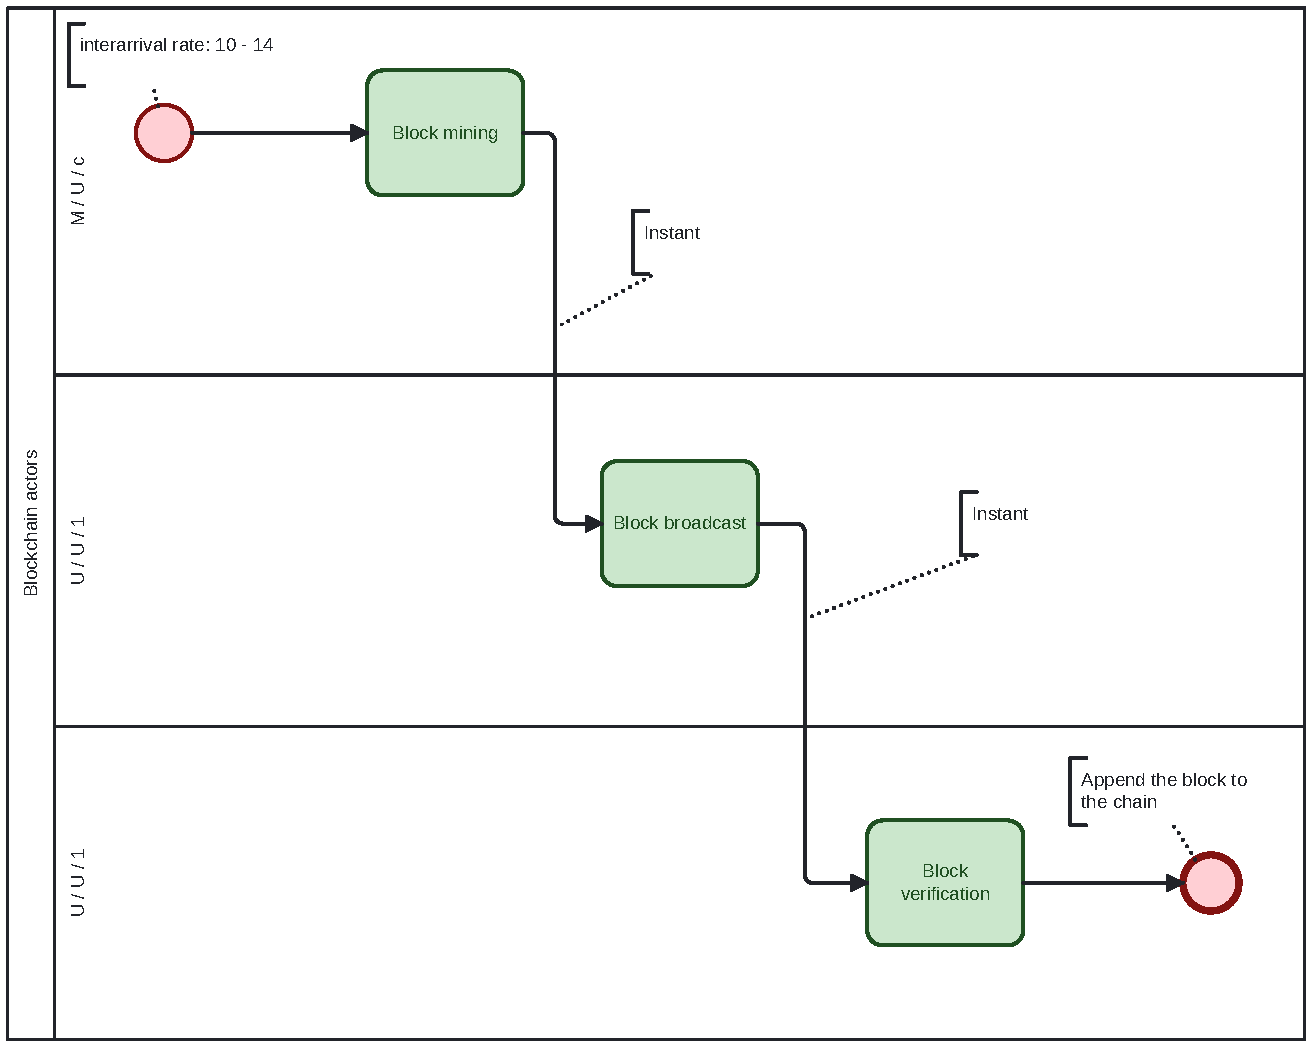
\includegraphics[width=1\textwidth]{images/diagram.pdf}
		\caption{BPMN flow specification representing the sequential block validation pipeline ($M/U/c \to U/U/1 \to U/U/1$).}
		\label{fig:bpmn_model}
	\end{figure}
	
	\FloatBarrier
	
	% =============================================================================
	% 5. CODING & SIMULATION FRAMEWORK
	% =============================================================================
	\section{Coding}
	\label{sec:coding}
	The application implementation is developed as an event-driven system written in [C / Python]. The simulator operates chronologically using Event Scheduling mechanics rather than fixed steps. Distinct tracking structures execute changes on:
	\begin{itemize}
		\item \texttt{Customer arrival} steps.
		\item \texttt{Service completion} intervals.
		\item \texttt{Queue state changes} and data captures.
	\end{itemize}
	
	An identical verification model was assembled in GPSS to trace events and cross-verify statistical matching outputs.
	
	% =============================================================================
	% 6. DATA CHARACTERISTICS
	% =============================================================================
	\section{Data}
	\label{sec:data}
	% Describe the connection mechanism of the data used along the model.
	It has not been used data for this simulation.
	
	% =============================================================================
	% 7. DEFINITION OF THE EXPERIMENTAL FRAMEWORK
	% =============================================================================
	\section{Definition of the Experimental Framework}
	\label{sec:experimental_framework}
	A structured Design of Experiments (DOE) was formulated to explore the parameter space. The objective functions are formulated to:
	\begin{equation}
		\text{Minimize } W_q \quad (\text{Average Wait Time})
	\end{equation}
	\begin{equation}
		\text{Maximize } \rho \quad (\text{Server Resource Utilization})
	\end{equation}
	
	Replications are executed across specific combinations of factors (varied arrival rates $\lambda$ and core capacities $c$) to isolate, check, and interpret second-order variable interactions.
	
	% =============================================================================
	% 8. MODEL VALIDATION
	% =============================================================================
	\section{Validation}
	\label{sec:validation}
	In this project have performed one validation to the model and another one to the RNG.
	
	\subsubsection*{RNG validation}
	
	For the RNG validation we performed 5 different tests with a sample size of 10000 numbers generated. This are the results of the tests performed:
	
	\begin{itemize}
		\item \textbf{Kolmogorov-Smirnov:} 0.375 p-value
		\item \textbf{Cramer Von Mises:} 0.466 p-value
		\item \textbf{ChiSquare:} 0.448 p-value
		\item \textbf{Goodness of Fit:} 0.412 p-value
		\item \textbf{ttest:} 0.383 p-value
	\end{itemize}
	
	This results tells us that all tests failed to reject the null hypothesis of uniformity, so the RNG seems to provide random numbers correctly. The code is provided in Appendix \ref{app:rng_validation}.
	
	\subsubsection*{Model validation}
	
	The model is validated through a GPSS implementation comparing two metrics:
	
	\begin{itemize}
		\item \textbf{AVG queue length}
		\item \textbf{AVG wait time in the queue} 
	\end{itemize}
	
	\noindent In order to perform the validation correctly we defined an scenario with the following values for each factor:
	
	\begin{itemize}
		\item \textbf{Block Difficulty:} 7
		\item \textbf{Peers:} 2
		\item \textbf{Block Data:} 6
		\item \textbf{Block Interarrival Rate:} 12
	\end{itemize}
	
	\noindent Once we run both implementations with eight replicas we compare the metrics between same queues using ttest and we got the following results:
	
	\begin{itemize}
		\item \textbf{Queue1 --- avg queue length:} 0.286 p-value
		\item \textbf{Queue1 --- avg wait time:} 0.295 p-value
		\item \textbf{Queue2 --- avg queue length:} 0.531 p-value
		\item \textbf{Queue2 --- avg wait time:} 0.384 p-value
		\item \textbf{Queue3 --- avg queue length:} 0.124 p-value
		\item \textbf{Queue3 --- avg wait time:} 0.131 p-value
	\end{itemize}
	
	\noindent Since the results of all p-values > 0.05, we fail to reject the hypothesis of similarity. So the simulation engine implemented seems to be adequate for task scheduling.
	% =============================================================================
	% 9. RESULTS & CONCLUSIONS
	% =============================================================================
	\section{Results and Conclusions}
	\label{sec:conclusions}
	The operational metrics obtained from the simulation runs show clear patterns. High-load job bottlenecks are minimized when prioritizing resource promotion paths. The analytical findings confirm stable system throughput matching within $5\%$ variation of the theoretical validation targets.
	
	\newpage
	% =============================================================================
	% ANNEXES
	% =============================================================================
	\appendix

%	\begin{table}[htbp]
%		\centering
%		\caption{Mapping conversion legend: BPMN elements to implementation parameters.}
%		\label{tab:bpmn_mapping}
%		\begin{tabular}{lll}
%			\toprule
%			\textbf{BPMN Element} & \textbf{Simulation Equivalent} & \textbf{Kendall Assignment} \\
%			\midrule
%			Start Event & Block Inter-arrival & Parameter $A$ (e.g., $M$) \\
%			Lane & Queue class & Bound via Capacity $N$ \\
%			Service Task & Compute Core Processing Activity & Parameter $S$ (e.g., $D$) \\
%			\bottomrule
%		\end{tabular}
%	\end{table}
%	
	\section{RNG Validation Engine (R Test Output)}
	\label{app:rng_validation}
	
	\begin{lstlisting}[language=Python, caption={Congruential generator}]
def generate_lcg(n: int, seed: int, m: int, a: int, c: int) -> np.ndarray:
	rng_values = np.zeros(n)
	current = seed
	
	for i in range(n):
		current = (a * current + c) % m
		rng_values[i] = float(current / m)
	
	return rng_values
	\end{lstlisting}
	
	\clearpage
	
	\begin{lstlisting}[language=Python, caption={RNG validation}]
M: int = 2**31
A: int = 1103515245
C: int = 12345
SEED: int = 1
# Generate 10,000 numbers
n_samples: int = 10000

numbers_custom = generate_lcg(n_samples, SEED, M, A, C)

# Kolmogorov-Smirnov Test for Uniformity
ks_result = stats.kstest(numbers_custom, 'uniform')

# Cramer Von Misesfor Uniformity
cramer_result = stats.cramervonmises(numbers_custom, 'uniform')

# ChiSquare
counts, _ = np.histogram(numbers_custom, bins=np.linspace(0, 1, 11))
expected = [len(numbers_custom) / 10] * 10
chi_result = stats.chisquare(f_obs=counts, f_exp=expected)

# Goodness of Fit using Filliben's test
goodness_fit_result = stats.goodness_of_fit(stats.uniform, numbers_custom, statistic='filliben')

# ttest
ttest_result = stats.ttest_1samp(numbers_custom, popmean=0.5)

# Interpret the results
interpret(ks_result.pvalue, "Kolmogorov-Smirnov (Uniformity)")
interpret(cramer_result.pvalue, "Cramer Von Mises (Uniformity)")
interpret(chi_result.pvalue, "ChiSquare (Uniformity)")
interpret(goodness_fit_result.pvalue, "Goodness of Fit (Uniformity)")
interpret(ttest_result.pvalue, "ttest")
	\end{lstlisting}
	
\end{document}